\documentclass{beamer}
\usepackage{amsmath}
\usepackage[english]{babel} %set language; note: after changing this, you need to delete all auxiliary files to recompile
\usepackage[utf8]{inputenc} %define file encoding; latin1 is the other often used option
\usepackage{csquotes} % provides context sensitive quotation facilities
\usepackage{graphicx} %allows for inserting figures
\usepackage{booktabs} % for table formatting without vertical lines
\usepackage{textcomp} % allow for example using the Euro sign with \texteuro
\usepackage{stackengine}
\usepackage{wasysym}
\usepackage{tikzsymbols}
\usepackage{textcomp}
% ELIMINAR COMANDOS DE NAVEGACION%%%%%%%%%%%
\setbeamertemplate{navigation symbols}

%\newcommand{\bubblethis}[2]{
 %       \tikz[remember picture,baseline]{\node[anchor=base,inner sep=0,outer sep=0]%
 %       (#1) {\underline{#1}};\node[overlay,cloud callout,callout relative pointer={(0.2cm,-0.7cm)},%
 %       aspect=2.5,fill=yellow!90] at ($(#1.north)+(-0.5cm,1.6cm)$) {#2};}%
 %   }%
%\tikzset{face/.style={shape=circle,minimum size=4ex,shading=radial,outer sep=0pt,
 %       inner color=white!50!yellow,outer color= yellow!70!orange}}

%% Some commands to make the code easier
\newcommand{\emoticon}[1][]{%
  \node[face,#1] (emoticon) {};
  %% The eyes are fixed.
  \draw[fill=white] (-1ex,0ex) ..controls (-0.5ex,0.2ex)and(0.5ex,0.2ex)..
        (1ex,0.0ex) ..controls ( 1.5ex,1.5ex)and( 0.2ex,1.7ex)..
        (0ex,0.4ex) ..controls (-0.2ex,1.7ex)and(-1.5ex,1.5ex)..
        (-1ex,0ex)--cycle;}
\newcommand{\pupils}{
  %% standard pupils
  \fill[shift={(0.5ex,0.5ex)},rotate=80] 
       (0,0) ellipse (0.3ex and 0.15ex);
  \fill[shift={(-0.5ex,0.5ex)},rotate=100] 
       (0,0) ellipse (0.3ex and 0.15ex);}

\newcommand{\emoticonname}[1]{
  \node[below=1ex of emoticon,font=\footnotesize,
        minimum width=4cm]{#1};}
\usepackage{scalerel}
\usetikzlibrary{positioning}
\usepackage{xcolor,amssymb}
\newcommand\dangersignb[1][2ex]{%
  \scaleto{\stackengine{0.3pt}{\scalebox{1.1}[.9]{%
  \color{red}$\blacktriangle$}}{\tiny\bfseries !}{O}{c}{F}{F}{L}}{#1}%
}
\newcommand\dangersignw[1][2ex]{%
  \scaleto{\stackengine{0.3pt}{\scalebox{1.1}[.9]{%
  \color{red}$\blacktriangle$}}{\color{white}\tiny\bfseries !}{O}{c}{F}{F}{L}}{#1}%
}
\usepackage{fontawesome} % Social Icons
\usepackage{epstopdf} % allow embedding eps-figures
\usepackage{tikz} % allows drawing figures
\usepackage{amsmath,amssymb,amsthm} %advanced math facilities
\usepackage{lmodern} %uses font that support italic and bold at the same time

\usepackage{tikz}

\usepackage{tcolorbox}

\usefonttheme[onlymath]{serif} %set math font to serif ones

\definecolor{beamerblue}{rgb}{0.2,0.2,0.7} %define beamerblue color for later use

%%% defines highlight command to set text blue
\newcommand{\highlight}[1]{{\color{blue}{#1}}}


%%%%%%% commands defining backup slides so that frame numbering is correct

\newcommand{\backupbegin}{
   \newcounter{framenumberappendix}
   \setcounter{framenumberappendix}{\value{framenumber}}
}
\newcommand{\backupend}{
   \addtocounter{framenumberappendix}{-\value{framenumber}}
   \addtocounter{framenumber}{\value{framenumberappendix}}
}

\newtcolorbox{boxA}{
    fontupper = \bf,
    boxrule = 1.5pt,
    colframe = black % frame color
}

%%%% end of defining backup slides

%Specify figure caption, see also http://tex.stackexchange.com/questions/155738/caption-package-not-working-with-beamer
\setbeamertemplate{caption}{\insertcaption} %redefines caption to remove label "Figure".
%\setbeamerfont{caption}{size=\scriptsize,shape=\itshape,series=\bfseries} %sets figure  caption bold and italic and makes it smaller


\usetheme{Boadilla}

\usepackage{hyperref}

% --------------------
% Overall information
% --------------------
\title[Economía I]{Economía I \vspace{4mm}
\\ Magistral 8: Las ganancias del comercio}
\date{}
\author[Riottini]{Franco Riottini}
\vspace{0.4cm}
\institute[]{Universidad de San Andrés} 

\begin{document}

\begin{frame}
\titlepage
\centering

\includegraphics[scale=0.2]{../Figures/logoUDESA.jpg} 
\end{frame}


\begin{frame}
\frametitle{¿Qué sucede cuando interactuamos con otros?}
\begin{itemize}
    \item En los modelos que vimos hasta ahora, las decisiones de los individuos no dependían de las decisiones de otros.
    \item Pero, ¡todo el tiempo interactuamos con otros seres humanos!
    \item La interacción genera distintos tipos de consecuencias, que afectan las decisiones de los demás individuos.
    \item ¿De qué modo la interacción afecta a los individuos? 
\end{itemize} 
\end{frame}

\begin{frame}
\frametitle{Especialización}
    \begin{itemize}
        \item ¿Conocen la historia de Robinson Crusoe?
        \item ¿Qué sucede cuando aparece Viernes?  
    \end{itemize}
    \centering \vspace{4mm}
    \begin{tabular}{|c|c|c|} \hline
    & Robinson Crusoe & Viernes \\ \hline
    Pescados por hora   & 4 & 3 \\ \hline
    Cocos por hora   & 6 & 2 \\ \hline     
    \end{tabular}
    \begin{itemize}\vspace{4mm}
        \item ¿Cuanto trabajan si quieren consumir 6 pescados y 6 cocos por día? 
    \end{itemize}
    \begin{boxA}
    \centering
    Una persona o un país tiene ventaja absoluta en la producción de
    un bien cuando puede producirlo en una menor cantidad de
    tiempo o con menos recursos que los demás.
    \end{boxA}
\end{frame}

\begin{frame}{Especialización}
    \begin{center}
        \begin{tabular}{|c|c|c|} \hline
            & Robinson Crusoe & Viernes \\ \hline
            Pescados por hora   & 4 & 3 \\ \hline
            Cocos por hora   & 6 & 2 \\ \hline     
        \end{tabular}
    \end{center}
    ¿Pueden hacer algo para mejorar su bienestar? 

    \begin{itemize}
        \item Costo de oportunidad de Robinson...
            \begin{itemize}
            \item De pescar en vez de recolectar cocos: $ 6/4 = 1,5 $ cocos por pescado 
            \item De recolectar cocos en vez de pescar: $ 4/6 =0,66 $ pescados por coco
            \end{itemize}
        \item Costo de oportunidad de Viernes...
            \begin{itemize}
            \item De pescar en vez de recolectar cocos: $ 2/3 = 0,66 $ cocos por pescado
            \item De recolectar cocos en vez de pescar: $ 3/2 = 1,5 $ pescados por coco
            \end{itemize}
        \item Para ver las ventajas del comercio y la especialización debemos comparar los costos de oportunidad de los bienes entre los individuos
    \end{itemize}
\end{frame}

\begin{frame}
\frametitle{Especialización}
    \begin{itemize}
        \item Costo de oportunidad de pescar en vez de recolectar cocos:
            \begin{itemize}
            \item Viernes: $ 0,66 < 1,5 $ Robinson 
            \end{itemize}
        \item Costo de oportunidad de recolectar cocos en vez de pescar:
            \begin{itemize}
            \item Viernes: $ 1,5 > 0,66 $ Robinson 
            \end{itemize}
        \item ¿Cuanto tiempo trabajan si se especializan?
            \begin{itemize}
            \item Robinson: Recoleta 12 cocos en 2 horas
            \item Viernes: Recolecta 12 pescados en 4 horas
            \end{itemize}
    \end{itemize}
    \begin{boxA}
        \centering
        Especializándose ambos en aquello para lo que
        son relativamente mejores, consiguen la misma cantidad de producción
        total y el tiempo de trabajo de ambos se reduce!
    \end{boxA}
\end{frame}

\begin{frame}{Ventaja Comparativa}
    \begin{itemize}
        \item ¿Como sabemos en que bien se tiene que especializar cada individuo?
        \begin{boxA}
            \centering
            Una persona o un país tiene ventaja comparativa en aquel bien
            cuyo costo de oportunidad es menor.
        \end{boxA}
        \item A pesar de que una persona o un país no tenga ventajas absolutas en ningún bien,
        siempre va a tener ventaja comparativa en alguno. 
        \item Al momento de comerciar, los países se van a especializar en la
        producción de aquellos bienes en los que tengan ventajas
        comparativas.
        \begin{boxA}
            \centering
            Con comercio, los precios relativos de equilibrio se encontrarán
            entre los costos de oportunidad de cada uno de los países.
        \end{boxA}
        \vspace{-4mm}
        \begin{equation*}
            2/3 = 0.66 \text{ cocos} < \text{ Precio del pescado } < 6/4 = 3/2 = 1.5 \text{ cocos}
        \end{equation*}
    \end{itemize}
\end{frame}

\begin{frame}
    \frametitle{Especialización}
    \begin{itemize}
        \item La división del trabajo (o especialización) permite aumentar la producción.
        \item Aprovechar la especialización es la clave del crecimiento económico (mundial).
        \item Explica los beneficios de la globalización.
        \item Pero ¿por qué difieren las productividades?

        \begin{itemize}
            \item Tecnologías distintas
            \item Heterogeneidad y ventaja comparativa (agentes difieren en habilidades o recursos, lo que los hace más o menos productivos en una actividad particular)
            \item Learning-by-doing (desarrollo de habilidades cuando se produce algo)
            \item Economías de escala (producir en grandes cantidades suele ser más costo-efectivo)
        \end{itemize}
        \item El estudio de los incentivos para el cambio tecnológico es un área importante de estudio para la economía
    \end{itemize} 
\end{frame}

\begin{frame}
    \frametitle{Un modelo Ricardiano simple}
    \begin{itemize}
        \item 2 países: Inglaterra y Portugal
        \item Dos productos: vino y telas
        \item Portugal tiene la ventaja absoluta en ambos.
        \item Inglaterra puede producirlos, pero Portugal tiene condiciones favorables tanto para producir uvas (para hacer el vino), como para criar ovejas (que dan la lana para las telas)
        \item Para Inglaterra es relativamente más difícil producir vino.
        \item Inglaterra tendrá una ventaja comparativa en la tela y se la exportará a Portugal
    \end{itemize} 
\end{frame}

\begin{frame}
    \frametitle{Un modelo Ricardiano simple}
    \begin{itemize}
        \item Supongamos que en Portugal (P) e Inglaterra (I) los bienes se producen sólo con trabajo (L), los trabajadores de cada país son:
        \begin{equation*}
            \begin{aligned}
                L_P & = 25 \\
                L_I & = 100
            \end{aligned}
        \end{equation*}
    \end{itemize} 
    \begin{center}
        \begin{tabular}{|c|c|c|} \hline
            & Portugal & Inglaterra \\ \hline
            Vino por persona   & 4 & 1 \\ \hline
            Tela por persona   & 2 & 1 \\ \hline     
        \end{tabular}
    \end{center}
    \begin{itemize}
        \item La productividad marginal del trabajo, entonces es:
            \begin{equation*}
                \begin{aligned}
                    PMgL_V^{P} = 4 \, &\, PMgL_T^{P} = 2 \\
                    PMgL_V^{I} = 1 \, &\, PMgL_T^{I} = 1
                \end{aligned}
            \end{equation*}
        \item ¿Cuáles son las posibilidades de producción de cada país?    
    \end{itemize} 
\end{frame}

\begin{frame}{Frontera de Posibilidades de Producción}
    \begin{itemize}
        \item Dada la cantidad de trabajadores y las productividades, podemos calcular cuanto produce un país si dedica todo su trabajo a un bien o a otro, o a una combinación de ambos.
        \begin{boxA}
            \centering
            La frontera de posibilidades de producción (FPP) muestra las combinaciones de bienes que un país puede producir con sus recursos y tecnología dados.
        \end{boxA}
    \end{itemize}

\end{frame}

\begin{frame}{Portugal}
    \centering
    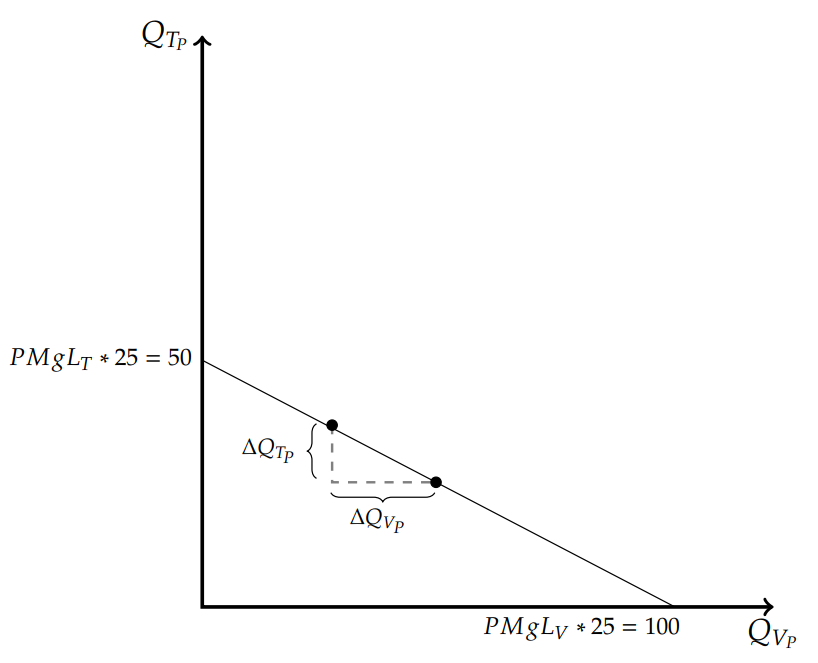
\includegraphics[scale=0.6]{../Figures/C18.2.png}
\end{frame}

\begin{frame}{Portugal}
    \begin{itemize}
        \item La pendiente de la FPP nos indica el costo de oportunidad de producir una unidad adicional del bien que está en el eje X\dots
        \item Si Portugal deja de producir 2 metros de tela, aumenta en 4 botellas la producción de vino.
        \item Entonces el costo de oportunidad para Portugal de producir vino en lugar de tela es de $2/4 = 0,5$ metros de tela por botella de vino.
        \[ \text{Pendiente} = \frac{\Delta Y}{\Delta X} = \frac{\Delta Q^{P}_T}{\Delta Q^{P}_V} = \frac{PMgL_T^{P}}{PMgL_V^{P}} = \frac{2}{4} = 0,5 \]
    \end{itemize}
\end{frame}

\begin{frame}
\frametitle{Eligiendo en Portugal}
\centering
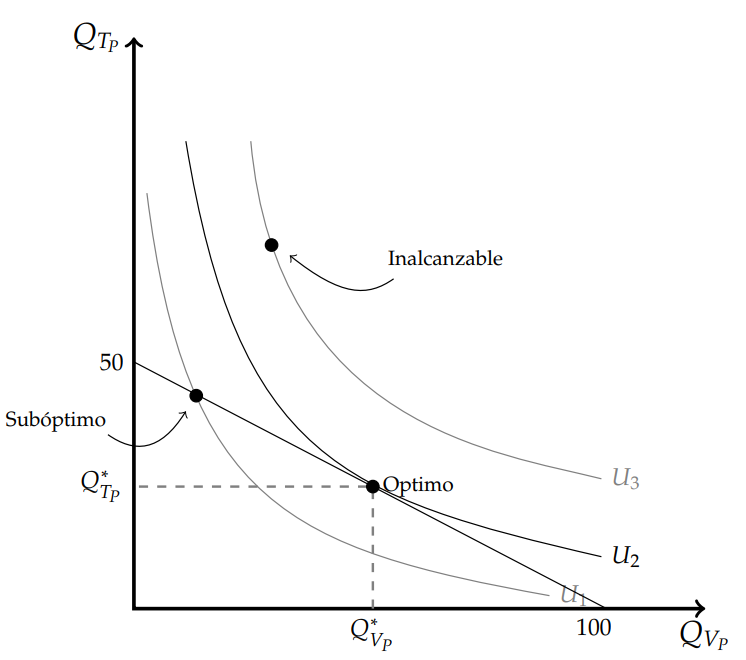
\includegraphics[scale=0.6]{../Figures/C18.3.png}
\end{frame}

\begin{frame}
\frametitle{Inglaterra}
\centering
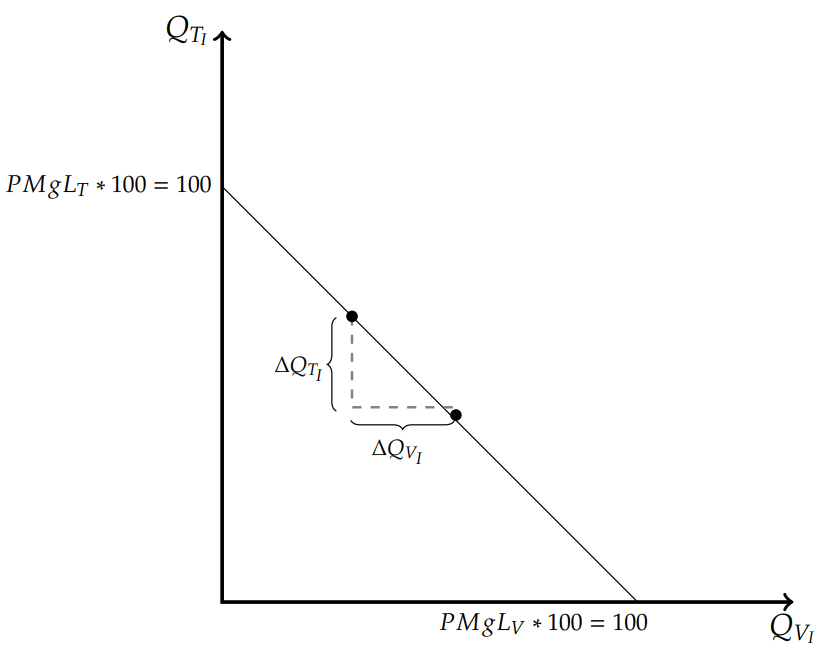
\includegraphics[scale=0.6]{../Figures/C18.4.png}
\end{frame}

\begin{frame}
\frametitle{Eligiendo en Inglaterra}
\centering
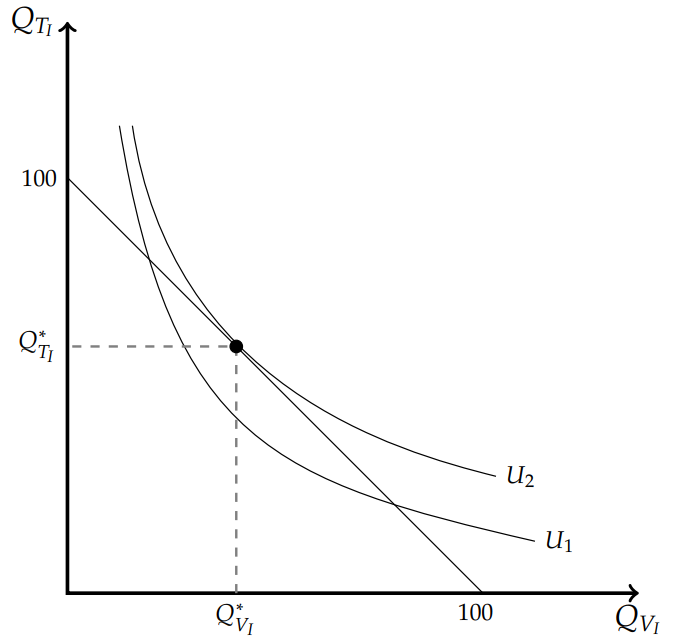
\includegraphics[scale=0.6]{../Figures/C18.5.png}
\end{frame}

\begin{frame}
    \frametitle{Ventaja comparativa}
    \begin{itemize}
        \item El costo de oportunidad varía entre los distintos países
        \begin{itemize}
            \item En Inglaterra le toma 1 trabajador producir 1 metro de tela o una botella de vino...
            \item ... pero en Portugal un trabajador produce 2 metros de tela o 4 botellas de vino.
        \end{itemize}
        \item Inglaterra tiene una ventaja comparativa en producir tela porque su costo de oportunidad en terminos de botellas de vino ($=1$) es menor que el de Portugal ($=2$)
        \item Portugal tiene una ventaja comparativa en producir vino porque su costo de oportunidad en terminos de metros de tela ($=0,5$) es menor que el de Inglaterra ($=1$)
        \item Permitiendo que los países comercien, cada uno se especializará en el bien en el que tiene \textbf{ventaja comparativa} y exportará al otro país la producción sobrante.
    \end{itemize}
\end{frame}

\begin{frame}
    \frametitle{La producción de Portugal}
    \centering
    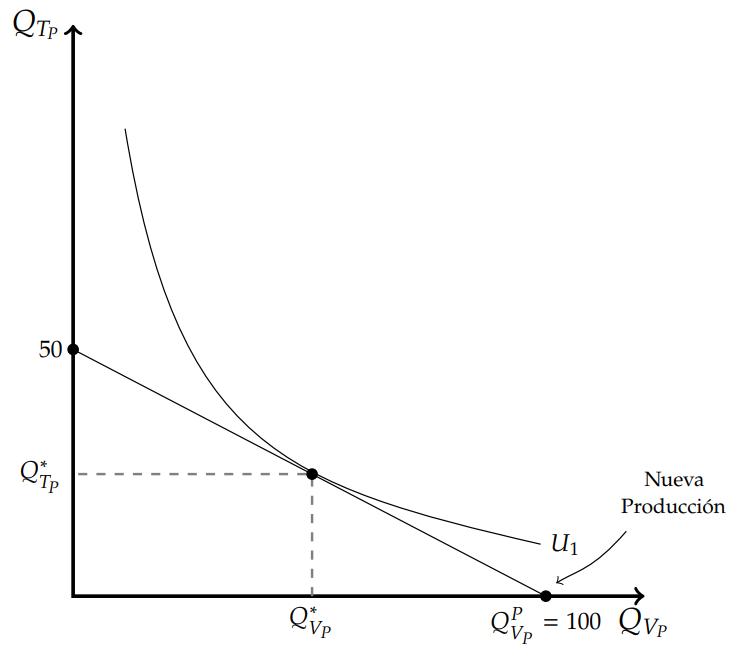
\includegraphics[scale=0.6]{../Figures/C18.6.png}
\end{frame}

\begin{frame}{Portugal cuando comercia}
    \begin{itemize}
        \item Esto nos dice que los precios internos van a ser distintos (pensemos en términos de un trueque!)
        \item Ahora que Portugal se especializa tiene dos opciones:
        \begin{enumerate}
            \item Sacrificar 1 botellas de vino para producir medio metro de tela (costo de oportunidad propio)
            \item Venderle a Inglaterra 1 botellas de vino pidiendole a cambio hasta un 1 metro de tela (que es lo que sacrificaría Inglaterra si quiere esa botella de vino).
        \end{enumerate}
        \item Inglaterra está en la misma, especializandose en la tela:
        \begin{enumerate}
            \item Sacrificar 1 metro de tela para producir 1 botella de vino
            \item Venderle a Portugal 1 metro de tela, pidiendole a cambio como mínimo 1 botella de vino pero como máximo 2 botellas de vino (que es lo que sacrificaría Portugal si quiere ese metro de tela).
        \end{enumerate}
        \item Esto es exactamente lo mismo que pensar que los precios en el otro país del bien que no produzco son menores.
        \item Si esto sucede, la FPP de ambos paises pivotea hacia afuera. 
    \end{itemize}
\end{frame}

\begin{frame}
    \frametitle{Portugal cuando comercia}
    \centering
    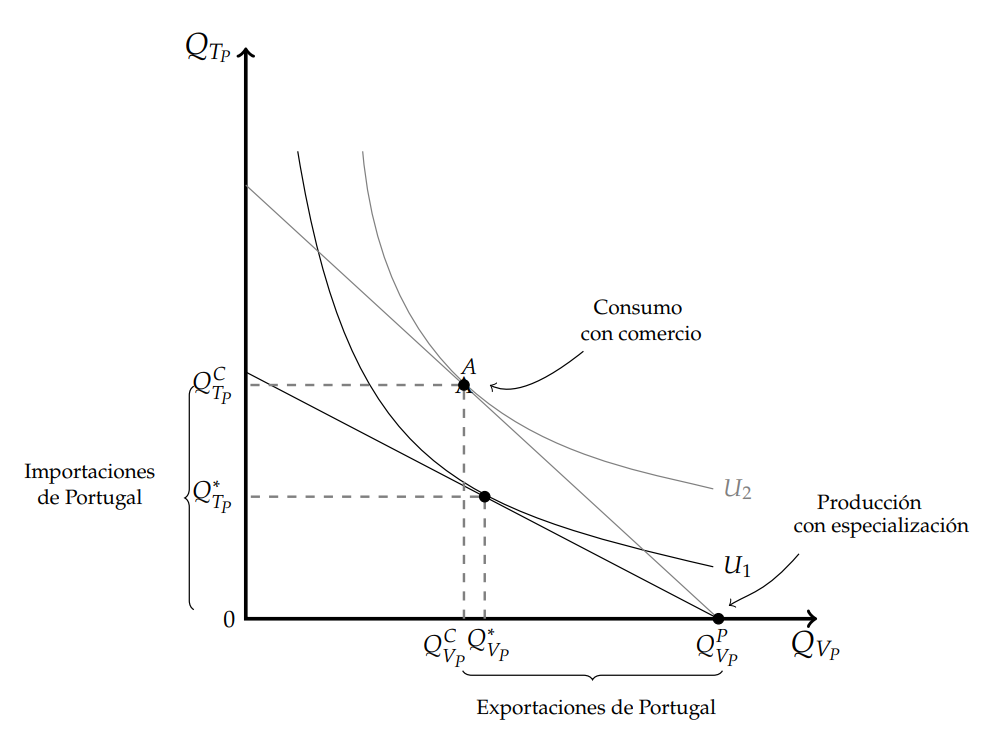
\includegraphics[scale=0.5]{../Figures/C18.7.png}
\end{frame}

\begin{frame}
    \frametitle{Inglaterra cuando comercia}
    \centering
    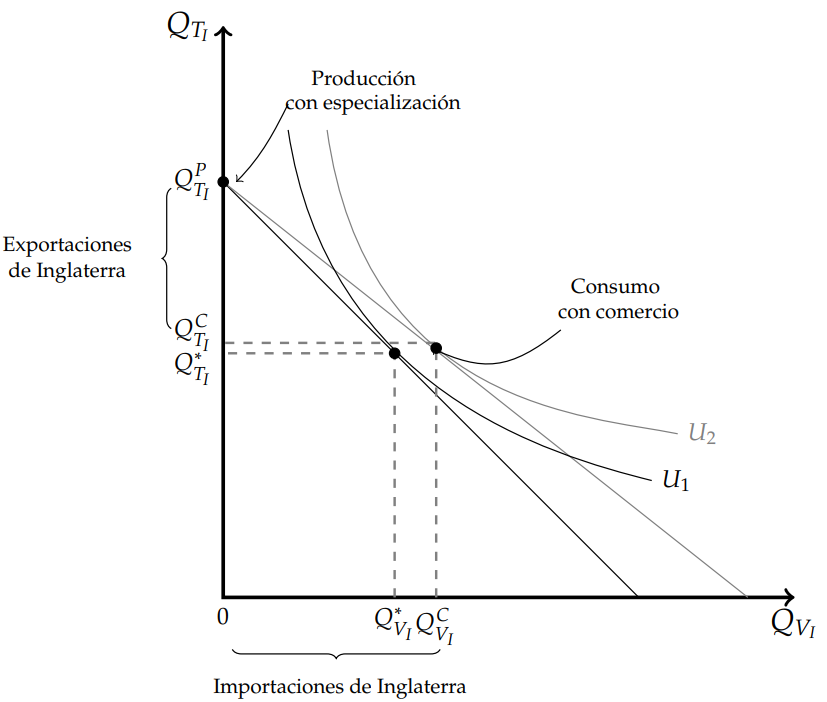
\includegraphics[scale=0.5]{../Figures/C18.8.png}
\end{frame}

\begin{frame}
    \frametitle{Conclusiones}
    \begin{itemize}
        \item No sabemos el precio al que se terminan comerciando los bienes porque queda indefinido.
        \item Aunque necesariamente estará entre la TMT de los dos paises.
        \item La presencia de mercados logra algo notable: cooperación no intencionada entre extraños.
        \item El libre comercio ejemplifica un juego en el que todos los participantes pueden beneficiarse de un escenario en el que todos ganan, todos cooperan para alcanzar el beneficio máximo.
        \item Esto es lo contrario de un juego de suma cero.
        \item La economía es la ciencia del "win-win".
    \end{itemize}
\end{frame}

\begin{frame}
    \frametitle{Conclusiones}
    \begin{itemize}
        \item A veces, por distintos motivos, la interacción social puede generar desvíos
        \item Una parte de la economía estudia este tipo de dilemas sociales.
        \item Principalmente cuando lo que tenemos son interacciones estratégicas.
        \item Parte de estos problemas que surgen en un mercado los vamos a estudiar más adelante.
        \item Para modelar cuando ocurren como resultado de interacciones individuales se suele utilizar lo que se conoce como teoría de juegos.
    \end{itemize}
\end{frame}


\end{document}